\documentclass{article}
\usepackage[utf8]{inputenc}
\usepackage{graphicx}
\usepackage{algorithm}
\usepackage[noend]{algpseudocode}

\title{A deconvolution model for linked-reads}
\author{Yoann Dufresne}
\date{April 2020}

\begin{document}

\maketitle

\begin{abstract}
Linked-read sequencing is an accurate and cost-effective alternative to long-read sequencing. DNA is cloned and cut into long molecules which are then sequenced using short reads. A sequence barcode is attached to each short read for the identification of its originating molecule. Due to experimental conditions, one barcode may correspond to multiple molecules. While these barcode collisions generally do not pose an issue when a reference genome is available, they complicate downstream reference-free analysis such as de novo assembly. This work aims to study this barcode collision problem, and propose an analysis framework that overcomes it in certain cases.
\end{abstract}


\section{Introduction}

%% Paul's intro START
A well-known limitation of short-read sequencing is that it does not provide long-range linking information, which is crucial to many studies.
There have been several techniques proposed to overcome this limitation, such as matepair libraries, which pair together distant reads, or longer reads, such as those produced by PacBio or Oxford Nanopore technologies.
Another approach, currently taken by  multiple approaches like 10x Genomics linked-reads, BGI single-tube long fragment read.
In linked-read sequencing, a genome, transcriptome or metagenome sample first undergoes special library preparation where DNA is cloned and cut into molecules of length 10-100 kbp.
Molecules are then isolated and sheared into shorter fragments and a barcode is attached to each short fragment for identification of its originating molecule.
Importantly, barcodes do not uniquely identify molecules: several molecules are typically labeled with the same barcode.
The fragments are then sequenced using a standard Illumina short-read protocol, where each molecule is sequenced at low coverage ($<$ 1x) but the overall coverage is high.
A similar technology enables single-cell transcriptome sequencing, which we do not focus on in this paper, where barcodes do not identify molecules but isolated cells, in order to simulate millions of single-cell experiments. %% Rayan: modified from Paul's intro as 'transcriptome linked-read' doesn't exist

Linked-reads have been used to assemble genomes \footnote{XXXXXXREFXXXXXXXX}, detect complex structural variants \footnote{XXXXXXREFXXXXXXXX}, and more
recently assemble metagenomes \footnote{XXXXXXREFXXXXXXXX}. A common challenge faced by most linked-read methods is that in order
to make use of the linking information, the reads within each barcode should be first separated into their
constituent molecules. The molecule separation problem is to replace the barcode identifiers of each read
with a molecule identifier. More formally, for each read r, we would like to find the identifier m(r) of its
originating molecule, given as input an observed identifier b(m(r)), where b(x) associates a barcode identifier
to a molecule x. Note that the image of b (all barcodes) is significantly smaller than its domain (all molecules),
hence b can be viewed as a non-invertible hash function. Currently, this problem is being tackled, one way
or another, as part of any method using linked-read data. However, formulating and solving this as an
independent problem can allow downstream methods to focus on their respective tasks, while assuming that
the reads have already been separated into molecules.

Molecule separation unlocks operations that are not possible with unseparated barcodes. For example,
in this paper we show how we can build a molecule overlap graph. Finding overlaps between reads sharing
two barcodes can also be framed as the detection of overlaps between the underlying molecules. Switching
from a read-centric or barcode-centric view to a molecule-centric view opens the possibility of using similar
methodology to long-read-overlap graphs. Molecule separation would also greatly facilitate and decrease
errors during the scaffolding stage of genome assembly. As noted by the authors of the ARCS scaffolder \footnote{XXXXXXREFXXXXXXXX},
different molecules having the same barcode can induce false joins in a scaffolding algorithm, resulting in
misassemblies.

The molecule separation problem can be tackled by aligning to a reference genome, if one is available.
Linked-read mapping tools such as longranger or ema \footnote{XXXXXXREFXXXXXXXX} are able to infer molecules by clustering mapping
locations of reads from the same barcode. While reference-based algorithms are often applicable, they do
not replace the need for de novo molecule separation algorithms. The quality of reference-based algorithms
is related to the quality of the assembly, since clusters cannot be identified across across different contigs.
When the genome or metagenome references are in a draft state, molecules will frequently span multiple
contigs, preventing their identification. Moreover, in many situations the reference is simply unavailable.
The de novo molecule separation problem has been previously studied in \footnote{XXXXXXREFXXXXXXXX}, where it was referred to as
barcode deconvolution. They first construct a bipartite graph between reads and barcodes. An edge (r, b) is
added when a k-mer of read r is found in another read of barcode b. Then a second graph is constructed with
reads as nodes, and edges indicating whether two reads are connected to sufficiently many common barcodes
in the bipartite graph. Finally, the second graph is clustered and each cluster reflects reads from the same
molecule. This algorithm was implemented in a single-threaded Python language prototype, Minerva. An
important limitation of Minerva is that its main data structure (the bipartite read-barcode graph) requires
$O(n)$ memory, where n is the number of reads. This is impractical for datasets with hundreds of millions or
billions of reads. Also, Minerva only uses shared k-mers between reads, and may fail to identify a molecule
if an insufficient number of reads share k-mers with reads from other molecules.


\subsection{From reads to graphs}
Forget reads, focus on long molecules. Presentation of the interval graph.
Explanation on merging barcodes (glued graphs) and transformation to intersection graph.
Definition of perfect merging, variable mergings and spurious interval graph.

\subsection{Definition of the 'bio' problems}
Here we can define multiple problem objectives.
\begin{enumerate}
    \item Counting problem: How many molecule present in each barcode ?
    \item Ordering problem: Is it possible to reconstruct the total order of molecules (intersection become interval graph) ?
    \item Reads assignation problem: Is it possible to assign reads to their original molecules (instead of barcodes) ?
\end{enumerate}


\section{Methods}

\subsection{Interval graphs}

A section that introduces interval graphs, intersection graphs, d-interval graph, and poses the problem of given a fusioned interval graph, how to 'de-fusion' it.

\subsection{Barcode graph structure}
Here we can focus on Cedric Analysis (O2, O3 and On ?).

\subsection{$d$-graphs: underlying local graph structure}
prerequisite to this section: Description of the merging process, underlying intersection graph, long molecule overlap efficiency. 

\subsubsection*{Local properties over fusion}

As first approximation, we suppose that our interval graph of molecules is perfectly homogeneous.
ie each molecule has the same size and the molecules are evenly distributed all along the genome.
This kind of structure is represented on the Fig-\ref{fig:fusion}-a (On top, the alignment of long molecules to genome G, on bottom, the molecule graph (MG) representing this alignment).\\
\textbf{Remark 1}: If each of the molecules is uniquely aligned on the genome, each node of the MG is strongly connected to local nodes and disconnected from the rest of the MG. More molecules are overlapping others, more the "edge thickness" is high.\\
\textbf{Remark 2}: Because the molecules are evenly distributed and are of the same size (except for the extrem positions on the genome), there is the same depth of molecules aligned on each genomic position. ie. there is the same number of edges for each node (except for the extreme ones). Choose one molecule, let's call \textit{depth} ($d$) the number of other molecules that overlap it on one position (If there is 4 molecules on a genomic position, $d=3$).

(here definition layout needed)We call $d$-graph an interval graph where $d$ is constant everywhere except for the $d$ leftmost and rightmost nodes.

During the sequencing process, having a barcode collision between two molecules means merging two nodes from the MG (Fig-\ref{fig:fusion}-b) into one node $c$ in the barcode graph (BG).
Because the MG is thick, even if the molecule information itself is lost during the merging process, the edges around $c$ are conserved.
These edges are clues to reconstruct the molecules.
If there is no other "local" fusion (ie no two molecules from the direct neighborhood of c are merging together), the molecule provenance information can be reconstructed by studying the edges.

\begin{figure}[htp]
    \centering
    \includegraphics[width=\textwidth]{fusion.pdf}
    \caption{ a. Representation of the interval graph from aligned molecules on genome (G) b. The fusion of two nodes (red barcode) from the molecule graph, preserve edge orientations in the barcode graph. }
    \label{fig:fusion}
\end{figure}


\subsubsection*{The building blocks of the $d$-graphs}

From a $d$-graph, extract a node (not in the $d$ nodes from the extreme positions in the graph), its $2\times d$ neighbors and all the induced edges.
We call this subgraph a \textit{unit $d$-graph} (udg).
Because we are in the perfect conditions, each of the nodes (excluding extreme nodes) induce an udg.
So udgs are the building blocks of a $d$-graph.

In the figure \ref{fig:perfect_udg}, we represented an extracted udg from its context.
From the bottom representation, we can see the different components of an udg.
First, an udg is composed of exactly $2\times d + 1$ nodes and centered on a node $c$.
All the other nodes are in the direct neighborhood of $c$ (the blue edges).
These $2 \times d$ nodes are 2 cliques of size $d$ (black edges).
Finally, the cliques are bounded together by what we call \textit{linking edges} (red edges).\\
\textbf{Remark}: From left to right on the representation, the linking edge number bounded to a node increase from 0 to $d-1$ before the central node ; then decrease from $d-1$ for the node just after $c$ to 0 for the rightmost node.
On total, there is exactly $\sum_{i=0}^{d-1}i$ linking edges in a udg.\\

\begin{figure}[htp]
    \centering
    \includegraphics[width=0.7\textwidth]{udg_composition.pdf}
    \caption{A unit 3-graph. Linear representation on top, unpacked representation on bottom. $c$ node is the central node. In black, the edges from the side cliques of the unit 3-graph. In blue, the edges between the central nodes and the other nodes. In red, the edges that bound the side cliques together.}
    \label{fig:perfect_udg}
\end{figure}

The representation of a $d$-graph as a succession of overlapping unit $d$-graphs is very important to transform the problem of "searching a $d$-graph into an intersection graph" to "searching a path into a set of unit $d$-graphs.
So, the first step to our $d$-graph reconstruction is to find a set of udgs inside of the BG.

\subsubsection*{Compute the udgs from a Barcode Graph}

The elements entering in the composition of a udg are used to extract them from their BG context.
For each node of the BG we apply the algorithm \ref{algo:udg}.

\begin{algorithm}
    \caption{Unit $d$-graph computation}
    \label{algo:udg}
    \begin{algorithmic}[1] % The number tells where the line numbering should start
        \Procedure{compute\_udg}{$n, d, BG$} \Comment{n: start node}
            \State $U \gets$ \O
            \State $nbs\gets BG.neighbors(n)$
            \State $subgraph \gets BG.induced\_subgraph(nbs)$
            \State $cliques \gets subgraph.cliques(d)$ \Comment{list cliques of size d}
            \For{$c1 \in cliques$}
                \For{$c2 \in cliques$}
                    \State $c \gets count\_links(c1, c2)$ \Comment{Count edges between the cliques}
                    \If{$c == \sum_{i=0}^{d-1}i$}
                        \State $U \gets U \cup udg(n, c1, c2)$ \Comment{Add the new udg}
                    \EndIf
                \EndFor
            \EndFor
            \State \textbf{return} $U$
        \EndProcedure
    \end{algorithmic}
\end{algorithm}


The central node is used to perform only a local search, the cliques are searched independently and the linking edges are used to confirm the presence of a unit $d$-graph.
If there is no local multiple fusion, this algorithm is sufficient to discover all the unit $d$-graphs (\textbf{Proof ?}).

\subsubsection*{Compute udgs on real Barcode Graphs}

Real barcode graphs are not exactly $d$-graphs.
The covering depth of the molecule and their size vary along the genome because of the sequencing methods.
The parameter $d$ is not constant all along the genome.\\
\textbf{Hypothesis 1}: it's more probable that $d$ smoothly vary along thousands of nucleotides rather than quickly drop or jump on a few base pair.\\
To avoid explicit use of the $d$ value in the udg computation process, we adapted algorithm \ref{algo:udg} to compute pseudo-udgs instead of perfect udgs.\\
\textbf{Hypothesis 2}: local max-cliques are a good proxy to $d$-cliques because the random fusion process should not repetitively merge together nodes from 2 (or more) local neighborhoods. Complete destructive fusions are highly improbable.\\
\textbf{Remark:} If the previous hypothesis is not true, there is a local critical merge.
The local information is lost and some udgs can't be computed but the other nodes can still be deconvoluted.

Without the $d$ value, we don't have a precise criteria to say that 2 cliques are the hands of a udg.
Instead, we score the approximated udgs by their linking edge count divergence from the count for an equivalent well balanced udg.
We use the algorithm \ref{algo:score} to score a pair of cliques.

\begin{algorithm}
    \caption{Divergence score between two cliques}
    \label{algo:score}
    \begin{algorithmic}[1] % The number tells where the line numbering should start
        \Procedure{div}{$c1, c2$} \Comment{cliques can be of different size}
            \State $d \gets max(|c1|, |c2|)$ \Comment{d used is the max length of cliques}
            \State $ref \gets \sum_{i=0}^{d-1}i$
            \State $obs \gets count\_links(c1, c2)$
            \State \textbf{return} $\sqrt{(ref - obs)^2}$ \Comment{Absolute difference}
        \EndProcedure
    \end{algorithmic}
\end{algorithm}

From this divergence score, one way to compute udgs is to fix a threshold and only generate a udg if its clique divergence is lower than that threshold.
But this solution is not sufficient to handle all $d$ values and variations.
Using it, results in producing too much or too few udgs regarding the threshold value.

\subsubsection*{Approximating the number of udgs}

To create only good udgs, we want to pair cliques that involve good divergence score.
So, first, from the list of all the max cliques computed on the neighborhood of a central node, we create a complete graph of cliques where the nodes are the cliques and the edges are weighted with the linked cliques divergence score (see figure \ref{fig:mwm}).\\
\textbf{Hypothesis 1}: No max clique is present inside of two different udg.\\
\textbf{Remark}: If the previous hypothesis is wrong for a $k$-clique, that means that in two different place of the genome, $k$ overlapping molecules share the same $k$ barcodes. It's highly improbable for large $k$ values.\\
\textbf{Hypothesis 2}: All the max cliques will be part of an interesting udg. This hypothesis is not totally true but will lead to an almost perfect solution that will be filtered in the following sections.

\begin{figure}[htp]
    \centering
    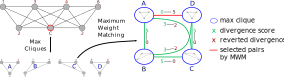
\includegraphics[width=\textwidth]{mwm.pdf}
    \caption{Max clique graph construction and maximum weight matching application}
    \label{fig:mwm}
\end{figure}

Regarding the two hypothesis, we created a udg factory based on the maximum weight matching algorithm.
This algorithm produce a matching in the graph, where the sum of all the selected edges weight is maximal.
In our clique graph we want the edges that are minimum.
So, we revert the maximum divergence order by doing $max\_div - div$ on each node. max\_div is the maximal divergence score on all the local clique pairs (see Fig. \ref{fig:mwm}).

\begin{algorithm}
    \caption{Approximate unit $d$-graph computation}
    \label{algo:audg}
    \begin{algorithmic}[1] % The number tells where the line numbering should start
        \Procedure{compute\_udg}{$n, BG$} \Comment{n: start node}
            \State $U \gets$ \O
            \State $nbs\gets BG.neighbors(n)$
            \State $subgraph \gets BG.induced\_subgraph(nbs)$
            \State $cliques \gets subgraph.max\_cliques()$ \Comment{list cliques of maximum size}
            \State $CG \gets clique\_graph(cliques)$ \Comment{Clique graph from divergences}
            \State $m = CG.maximum\_weight\_matching()$
            \For{$(c1, c2) \in m$}
                \State $U \gets U \cup udg(n, c1, c2)$ \Comment{Add the new udg}
            \EndFor
            \State \textbf{return} $U$
        \EndProcedure
    \end{algorithmic}
\end{algorithm}

The final algorithm to compute the approximate unit $d$-graphs is presented in algorithm \ref{algo:audg}.
It is now totally independent of the $d$ values.
The usage of a maximum weight matching on our clique graph generate high quality udgs but don't have a guaranty on correctness of those udgs.

Local search for linked cliques are a kind of local graph community detection.
More than classical clustering, the max clique detection allow to include some nodes in multiple communities.
This property leads to a udg detection algorithm very resilient to multiple local merges.
But because we use a heuristic to generate udgs some of them are wrong and others are missing.

\subsection{$d^{2}$-graph: Connecting unit $d$-graphs}

In this section, we will use unit $d$-graph or udg as language shortcut for what we called approximate unit $d$-graph in the previous sections.
We will use \textit{perfect udg} for a well balanced and 0 divergence udg.

udgs are local structure defined in a node neighborhood in the barcode graph.
Because we know that the barcode graph is originated from an intersection graph, we should be able to find a succession of udg that cover our genome from the beginning to the end.
In fact, if we are in the perfect case, the genome should be a succession of perfect udgs where two successive udg share exactly $2 \times d$ barcodes.
Each of the two udgs will have one barcode that is not in the other.
We can call these two nodes \textit{extreme nodes}.

\begin{figure}[htp]
    \centering
    \includegraphics[width=0.6\textwidth]{overlap.pdf}
    \caption{Unit $d$-graph overlap}
    \label{fig:overlap}
\end{figure}

A real barcode graph is a bit more messy and two successive udgs can have different sizes, share less than $2 \times d$ barcodes and have more than 2 extreme nodes (Fig \ref{fig:overlap}.
But the idea remain the same, we should be able to go from the first udg (regarding the genomic position) to the last one by successive overlaps.

To support this traversal operation, we create a graph of unit $d$-graphs that we call $d^2$-graph (d2g).
In this graph, the nodes are the udgs generated by the algorithm \ref{algo:audg} and the edges are weighted edges between udgs that share at least one barcode.
The weight (distances) are defined as the number of barcodes that are extreme nodes separating the udgs pairs (Fig \ref{fig:overlap}.

TODO: Voir avec Rayan pour utilisation threshold/moyen plus malin.


Interesting assembly properties.
Cedric work on path retrieving ?
conclusion: More interesting solution for counting problem (filter out a lot of wrong udgs).
Assembly process allow to traverse the graph and try to extract total order.

\section{Results}

\subsection{Interval graphs}

Yoann's simulations where we started from overlap graphs

\subsection{Genome graphs}

Rayan's section where we take real E.coli molecules.

A figure I want to see: Quality of d2-graph (need to find a metric) versus number of fusions (~ average number of molecules per barcode).

\section{Conclusion}

\end{document}
